\subsection{Ejercicio 6}
\graphicspath{ {img/06} }

GPG, o GnuPGP, es la implementación de GNU del estándar de criptografía PGP. Con el comando \texttt{gpg} se pueden generar y gestionar claves, firmar, cifrar, descifrar y comprobar la firma de documentos encriptados con PGP.

Para generar un par de claves se puede utilizar el siguiente comando:
\begin{minted}[
    frame=single,
    framesep=8pt,
    breaklines,
    bgcolor=bgGray
]{bash}
    gpg --gen-key
\end{minted}

que preguntará información sobre el usuario para generar la clave, concretamente:
\begin{itemize}
    \item{Nombre}
    \item{Dirección de correo electrónico}
    \item{Contraseña para las claves}
\end{itemize}

Sin embargo, en la captura se muestra la generación de las claves con \\ \texttt{gpg --full-gen-key}, que permite generar la clave de manera más configurable, indicando también el algoritmo de las claves y la caducidad de las mismas

\begin{figure}[H]
    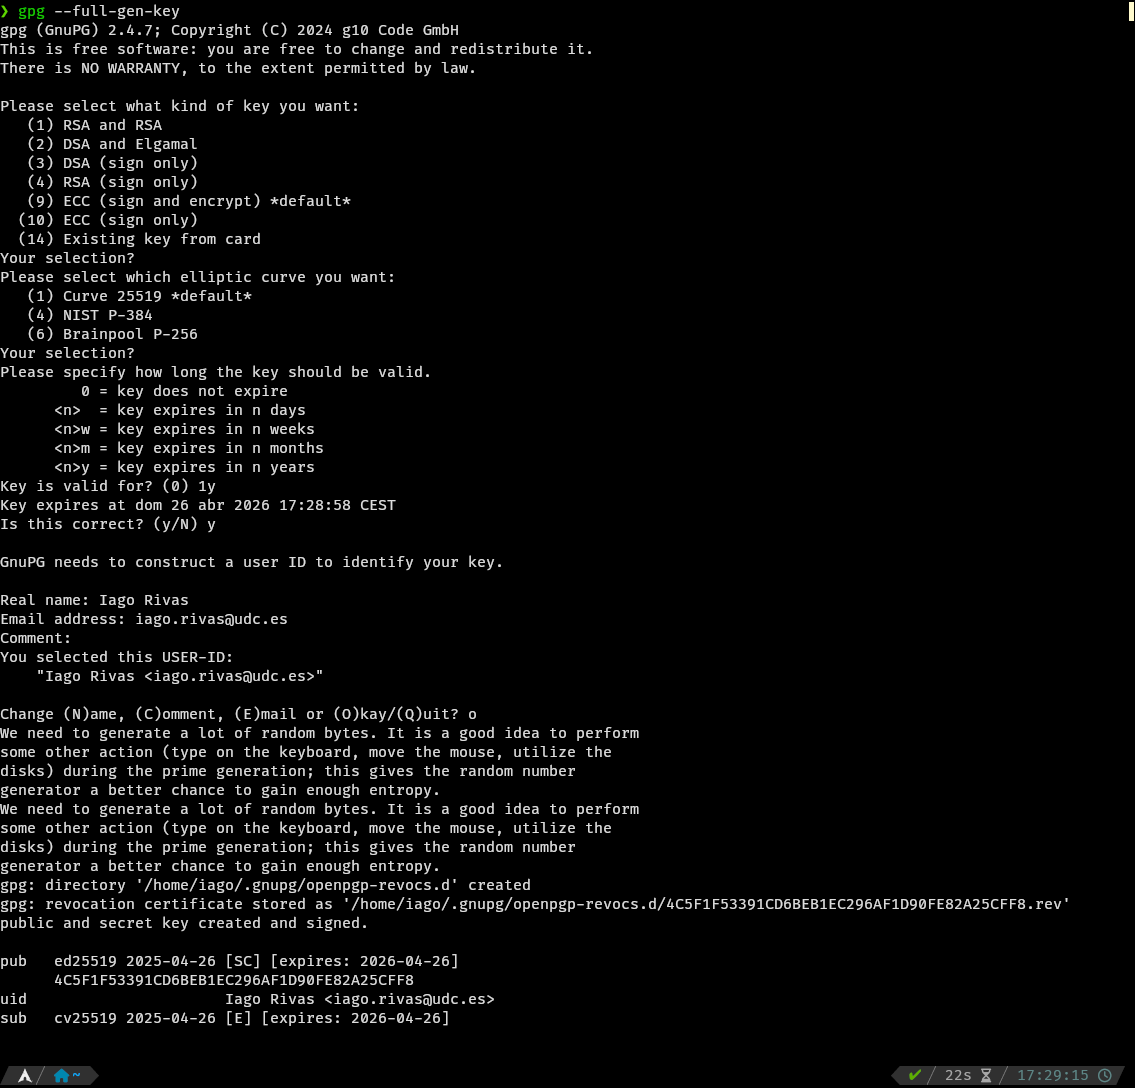
\includegraphics[width=\textwidth]{gpg-genkey.png}
    \caption{Generación del par de claves con \texttt{gpg}}
\end{figure}

Debido a la versatilidad de la criptografía de clave pública, no es neceario que todas las partes tengan claves generadas con el mismo algoritmo. En la captura se selecciona una clave de curva elíptica, pero es perfectamente factible que otra de las claves del grupo utilice RSA, ya que en ningún momento se usan las claves de más de una parte a la vez, se cifra con la clave pública del destinatario y se cifra con la privada del remitente.

Una vez generadas las claves, es necesario exportarlas, para poder compartirlas. Thunderbird comparte automáticamente la clave pública al enviar un correo, pero necesitaremos las claves públicas del resto de integrantes para poder empezar la conversación. Para exportar las claves se puede utilizar el comando:

\begin{minted}[
    frame=single,
    framesep=8pt,
    breaklines,
    bgcolor=bgGray
]{bash}
    gpg --output 1.2_Rivas_Moar,_Iago.asc --armor --export iago.rivas@udc.es
\end{minted}

La opción \texttt{--armor} hace que se exporte una representación en ASCII de la clave, y simplemente es necesario indicar la clave que se quiere exportar por su correo electrónico o con el ID. Compartir la clave sería cuestión de enviarla por correo electrónico u otro medio. Para importar una clave pública se puede utilizar la opción \texttt{import}:

\begin{minted}[
    frame=single,
    framesep=8pt,
    breaklines,
    bgcolor=bgGray
]{bash}
    gpg --import 1.2_Losada_Sanchez,_Alicia.asc
\end{minted}

Si quisiéramos copiar el par de claves completo a otro ordenador, para poder utilizarla en varios ordenadores, tendríamos que cambiar \texttt{--export} por \texttt{--export-secret-keys}. También necesitaremos el par completo para poder importarlo en Thunderbird.

\begin{figure}[H]
    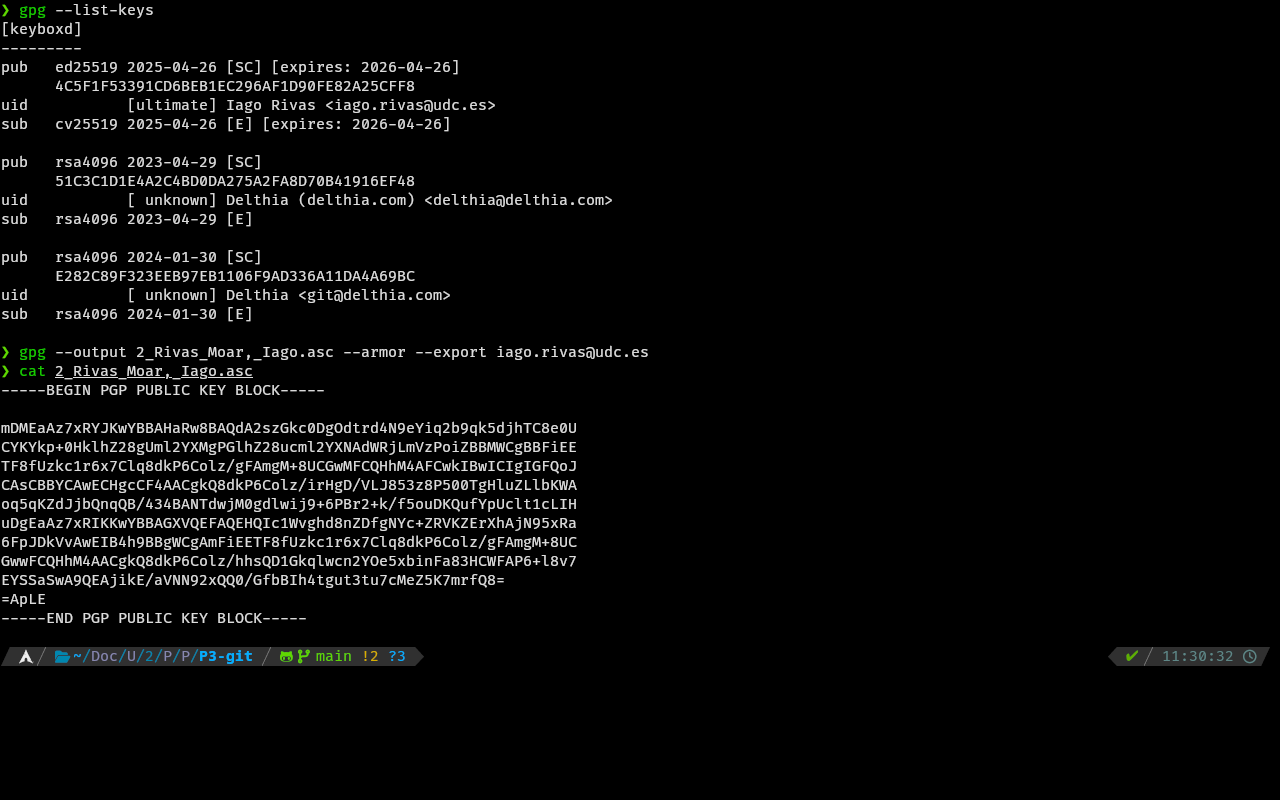
\includegraphics[width=\textwidth]{gpg-export.png}
    \caption{Exportación de la clave pública}
\end{figure}

Por último, si perdiéramos el control de nuestra clave privada y quisiéramos revocarla, utilizaríamos el comando

\begin{minted}[
    frame=single,
    framesep=8pt,
    breaklines,
    bgcolor=bgGray
]{bash}
    gpg --output iago.rivas-revocation.asc --armor --gen-revoke iago.rivas@udc.es
\end{minted}

Que generaría un comando de revocación que podríamos compartir con nuestros contactos.
